\textbf{El número de medallas de plata ganadas por Japón.}\vspace{.3cm}

Para resolver esta consulta, primero identificamos la necesidad de acceder a la información sobre la nacionalidad de los atletas y el tipo de medalla ganada. Por lo tanto, estructuramos nuestra consulta de la siguiente manera: \vspace{.3cm}

\begin{lstlisting}
    SELECT 
    COUNT(*) AS medallas_plata
FROM 
    Medalla m
JOIN 
    Atleta a ON m.IDAtleta = a.IDAtleta
WHERE 
    a.Nacionalidad = 'Japonesa' AND m.TipoMedalla = 'Plata';
\end{lstlisting}

 \vspace{.3cm}

Primero, seleccionamos la tabla Medalla y la aliasamos como m. Luego, realizamos un (JOIN) con la tabla Atleta, aliasada como a, utilizando la columna IDAtleta que es común en ambas tablas. Por lo cual dado este join, se nos permite acceder a la información de los atletas que han ganado medallas. \\

Despues, seleccionamos la tabla Medalla para contar cuántas medallas de plata ha ganado Japón. Utilizando la función COUNT(*) para contar todas las filas que cumplen con las condiciones especificadas en el WHERE, es decir, aquellas donde la nacionalidad del atleta es 'Japonesa' y el tipo de medalla es 'Plata'. \vspace{.3cm}

El resultado es un único valor que representa el total de medallas de plata ganadas por Japón ya que es lo unico que se nos pide \textit{(el número de medallas de plata ganadas por Japón)}. \vspace{.3cm}

\textbf{Resultado:}
\begin{center}
    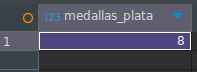
\includegraphics[width=10cm]{resources/resultados/r7.png}
\end{center}   

Nota: Para obtener este resultado, se añadieron manualmente registros en la tabla Medalla para asegurar que Japón tenga medallas de plata registradas. \vspace{.3cm}